\title{Lab 1: Arduinos \& LEDs}
\author{Winter 2018}
\date{January, 2018}
\documentclass[12pt]{article}
\usepackage[margin=1in]{geometry}
\usepackage{graphicx}
\usepackage{circuitikz}
\usepackage{fancyhdr}

\chead{Written and Edited by Arun Nagpal, Aaron Ridley, Scott Smith,
  and Lyndon Shi}

\usepackage{hyperref}

\begin{document}
	\maketitle
	\thispagestyle{fancy}
	
	\section*{Materials}
	\begin{itemize}
		\item 1 \quad Arduino Nano
		\item 9 \quad LEDs
		\item 3 \quad 1-k$\Omega$ Resistors
		\item 3 \quad 2-k$\Omega$ Resistors
		\item 3 \quad 7.5-k$\Omega$ Resistors
		\item 3 \quad 10-k$\Omega$ Resistors
	\end{itemize}
	
\section*{Introduction}

Welcome to ENGR100-950! Over the course of the next couple of weeks,
you will be designing and building your own circuit board, complete
with measurement instruments to make measurements of all sorts of
atmospheric variables.\\
	
In lecture, you've had a crash course on the ins and outs of
Microcontrollers. Now, you'll be working with your own \textbf{Arduino
  Nano} in order to get used to using these devices. The Nano will be
the brain of your payload, and is very well-suited to these sorts of
applications, as you will see.\\
	
The \textbf{input/output (IO) pins} on the Nano each serve different
purposes. On the next page, there's a helpful diagram that details the
types of pins on the board.\\
	
\begin{figure}[h]
  \begin{center}
    \includegraphics[width=\linewidth]{Figures/Nanopinout.png}
    \caption{Photo Credit: forum.arduino.cc}
  \end{center}
  \label{nano}
\end{figure}

In general, the digital pins are on one side (D2-13), and the analog
pins are on the other (A0 - A7). Digital pins read and write binary
values - HIGH (5V) or LOW (0V) - while analog pins are
\textbf{read-only} and read analog values from 0V - 5V. Read-only
means that you can't arbitrarily set an analog value to an analog pin,
you can only read the voltage that it `sees' on the circuit or sensor
you connect it to. \\

Finally, it's worth noting the GND pin. Voltage values are read with
respect to some constant reference. They are \textbf{relative}, not
\textbf{absolute}. This reference is usually called 'Ground.' There
should ALWAYS be a ground connection on every circuit you make,
whether you’re using a microcontroller or not. This is essential when
dealing with electricity, to make sure that things don't spark or get
fried because they draw too much power.\\

To illustrate, consider the simple LED circuit shown in Figure~\ref{led},
where a 5V supply powers a bulb, which is attached to GND. The two
circuits shown in Figure~\ref{led} are actually equivalent. In the circuit on
the left, the 5-volt battery raises the top half of the loop 5 volts
higher than the bottom half. The bottom half of the loop is held at
zero volts, since it is grounded. Current flows clockwise from the
positive (top) to the negative (bottom) terminals of the battery.\\
    
\begin{figure}[h]
  \begin{center}
    \begin{circuitikz} \draw
      % First circuit
      (0, 0)	to [battery1, label={5V Batt.}]	(0,4) 
      (0, 4)	-- (4, 4)
      (4, 4)	to [full led, *-*]	(4, 0) -- (0, 0)
      (2, 0)	node[ground, label={[label distance=0.8cm]below:GND}]{}
      % Second circuit
      (7, 0)	node[ground, label={[label distance=0.8cm]below:GND}]{}
      (7, 4)	to [full led, o-*]	(7, 0)
      (7, 4)	node[label={above:5V}]{}
      ;
    \end{circuitikz}
  \end{center}
  \caption{A simple circuit powering an LED}
  \label{led}
\end{figure}
	
In the circuit on the right, the top node is held at 5V by some unseen
source, and the bottom is held at 0V because it is grounded. The
current flows down, into the grounded node. This representation works
great if you want to analyze a fragment from a larger circuit.
	
\section{The Breadboard}
	
Before actually launching into the building of circuits, it's
important to understand the tools that you are working with. Your
breadboard will act as the `circuit board' on which you build your
systems. Notice that it is organized by enumerated rows and columns.
	
The pins of the electronic devices go into the holes in the
breadboard. These holes are related to each other in that every row of
5, as defined on the board, are electrically connected. This means
that if, for instance, you connect a 5V battery to a given hole, all
of the holes in that row are raised to 5V.

\begin{figure}[h!]
   \begin{center}
     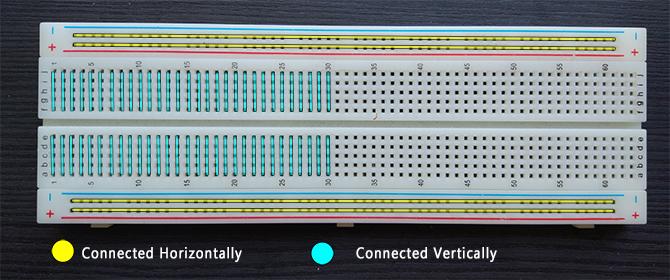
\includegraphics[width=\linewidth]{Figures/breadboard_annotated_670-1.jpg}
     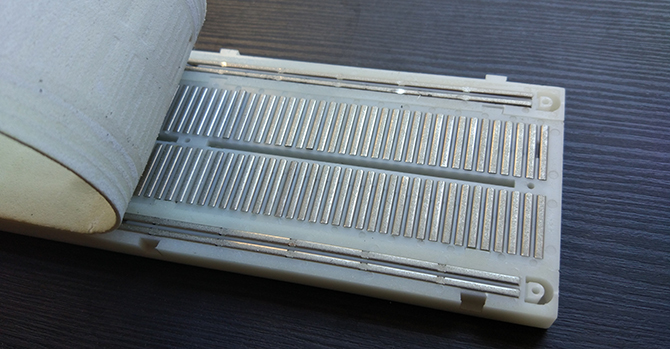
\includegraphics[width=\linewidth]{Figures/breadboard_back_peel_670.jpg}
     \caption{A breadboard, annotated (above) and with the plastic cover removed (below).\newline  \href{https://www.makeuseof.com/tag/what-is-breadboard/}{Credit: Makeuseof.com}}
   \end{center}
\end{figure}
    	
The little legs on the Arduino are called \textbf{headers}, which are
metal pins that can be inserted into the breadboard. The LEDs and
resistors that you’ll use today are also made in a form that can be
used with a breadboard. You'll be building the circuit show in Figure
2 momentarily. \newline
    	
Pause and check-in with your group. What questions do you have about
breadboards? What do you think an advantage is of prototyping with a
breadboard is? Even if you have not worked with electronics before,
can you think of any disadvantages?


Circuit elements are connected in breadboards by connecting the input
pins of one device to the same row as the output pins of another
device. In this way, devices can be chained together to create complex
circuits. An example is shown below (Fig. 3). This circuit is called a
voltage divider, and consists of two resistors connected end to end. A
formal circuit diagram of a voltage divider is shown later in this
manual (Fig. 4).
	
\begin{figure}[h]
  \begin{center}
    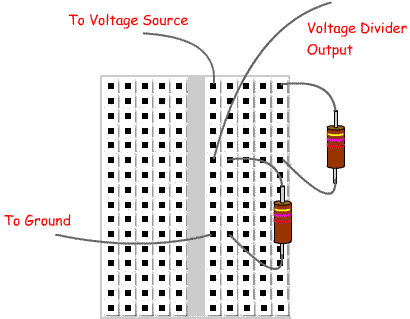
\includegraphics[width=\linewidth]{Figures/voltagedivider.png}
    \caption{Photo Credit: electroschematics.com}
  \end{center}
\end{figure}
	
\subsection*{Arduino Blink}
Let’s try making first contact with the Arduino!
\begin{enumerate}
	
\item Insert the Arduino into the breadboard. Don't add the LED and
  resistor just yet. Notice how it sits over the gap between the two
  columns on the breadboard. This positioning is intentional - if we
  placed the Arduino on one side of the breadboard, we would be
  electrically connecting pins on either side of the device. We don't
  know what this would do, and we want to make room to plug in other
  electronic devices, so as a result we place the Arduino in the
  center of the breadboard.
		    
\item Turn on the Arduino by plugging in the micro USB cable into the
  device and the USB cable into your computer. Note that an LED built
  into the device should begin glowing.
		    
\item Load the Arduino Blink sketch in your IDE (sketch = nickname for
  an Arduino program).

  \begin{enumerate}
  \item If you downloaded the Arduino Integrated Development
    Environment (IDE), first specify the Arduino model that you are
    working with by navigating to Tools $\rightarrow$ Board
    $\rightarrow$ Arduino Nano 33 BLE. Now, go to File $\rightarrow$
    Examples $\rightarrow$ Basics $\rightarrow$ Blink.
        		    
  \item If you are using the Arduino Web Editor, first specify the
    Arduino model that you are working with by navigating to the
    dropdown menu labeled \textbf{Select Other Board \& Port}. Search
    and select \textbf{Arduino Nano 33 BLE}. Now, look to the left
    hand side and navigate to Examples $\rightarrow$ Basics
    $\rightarrow$ Blink.

  \end{enumerate}
    	        
\item A new window should open up, with some code in it. In the
  lefthand corner of that window, click the checkmark to
  \textbf{compile} the program, and then click the arrow to
  \textbf{upload} the compiled program to the Arduino. Observe what
  happens on your Arduino.

  \textbf{ Troubleshooting:} If another LED on your Arduino does not
  begin blinking, try adjusting these settings, and then ask an IA:
    
  \begin{enumerate}
  \item If you downloaded the Arduino IDE, go to Tools $\rightarrow$
    Port and select a different USB port on your computer, then
    re-upload the program. Try this on all available ports.
  \item If you are using the Arduino Web Editor, go to \textbf{Select
    Other Board \& Port} and select a different port for the Arduino
    Nano.
  \end{enumerate}
	   
\end{enumerate}


\subsection*{Arduino Programming Basics}
Let's walk through the elements of the Arduino Blink sketch that you
just ran. Every Arduino sketch consists of two functions:
\verb|setup()| and \verb|loop()|. Try opening a new Arduino sketch
(File $\rightarrow$ New) and you’ll notice that these functions are
always provided to you as the starting point.
        
\begin{itemize}
\item The \verb|setup()| function runs once when you upload a sketch
  to the Arduino, power the board, and/or press reset (see if you can
  find the reset button on your Arduino).
        
\item The \verb|loop()| function runs “over and over again forever” –
  or at least until you upload different code or remove it from its
  power source.
\end{itemize}

The Arduino stores the most recent program that has been uploaded to
it in it’s memory. See this for yourself by unplugging the Arduino
from your computer, plugging it back in, and watching it restart the
activities from the Blink sketch Even though you can't see it
happening on the hardware, the Arduino ran the \verb|setup()| function
once and then proceeded to continuously run the \verb|loop()|
function.
        
Pause here and discuss with your partner(s): In an Arduino sketch,
what kinds of actions belong in a \verb|setup()| function versus a
\verb|loop()| function?
        
The last bit of the Arduino IDE that should be highlighted is the
black box at the bottom of the window known as the \textbf{terminal}.
By now you've already seen a success message appear after the Blink
sketch. Perhaps while getting that sketch to run, you saw some error
messages in the terminal as well. Although at first glance the error
messages can be nasty, they can be \textit{very} useful when
debugging. Other programmers have crafted these messages to help you
figure out what has gone wrong in your program. When you don't know
where to begin, try pasting that error into your favorite search
engine. There's a decent chance that you aren't the first one to
encounter this error!

\subsection*{Arduino Documentation}
As stated in the prelab, Arduino refers to a company that manufactures
open-source electronics and the community of people that provide ways
to use those electronics.

The Arduino IDE provides a wide range of functions that can be used in
your Arduino programs. All of these functions are documented on the
Arduino website. Reading documentation to understand and use something
made by someone else is a really important skill in engineering. Look
up \verb|pinMode()|, \verb|digitalWrite()|, and \verb|delay()| on your
favorite search engine and read the documentation. Between looking up
functions, discuss how these functions are used in the Arduino Blink
program.

        
\subsection*{LED Blink}
Now we'll see how we can control an external LED using an Arduino.
\begin{enumerate}
\item Unplug your Arduino from your computer. It is good practice to
  never manipulate a circuit while power is being supplied to it.
\item Build the LED circuit shown in Figure 2.
        	
\item Plug your Arduino back into your computer. 
        	
\item Notice that only the Arduino’s built-in LED is blinking. Let’s
  add some code to the Blink sketch so that both the Arduino’s LED and
  this new LED cooperate. Look at your circuit. Following the picture,
  you should have connected the LED to one of the Arduino’s 14
  \textbf{digital} pins, which are labelled D1-D14. Figure out which
  digital pin your LED is connected to, and then add a line of code in
  the \verb|setup()| function to initialize the LED using the command
  \verb|pinMode(<Your pin number>, OUTPUT)|;
        	
\item Follow the same logic to add lines of \verb|digitalWrite()| for
  this additional LED to the \verb|loop()| function of your program.
        	
\item Test this code and make sure that both LEDs blink. Be aware that
  LEDs only turn on when placed in your circuit in the correct
  orientation. Try switching the orientation of your LED if it doesn't
  turn on at this point. Take note that one leg of the LED is longer
  than the other. This can help you remember the proper orientation in
  the future.
        	
\item Save your code and rename it to something more recognizable. It
  will be prudent to create a new folder on your computer to store
  these scripts for easy recollection later. You will be submitting
  this program, so make sure to keep it.
        	
\end{enumerate}
        
\subsection*{Knight Rider}
Connect 8 more LEDs to the Arduino digital out pins and ground them
with one resistor, like in Figure 3. Write a new Arduino script to
approximate the behavior of the light in the beginning of the video
below (so that the light shifts left and right at a constant
speed). This program should be written with less than 20 lines in
loop. Make sure to save this code, as you will be submitting it. You
should have three separate programs saved so
far. (\url{https://www.youtube.com/watch?v=FpyKlLuLbcs})
        



        
	\section{Voltage Divider}
	Consider a \textbf{voltage divider} shown below. The output voltage is related to the input voltage through the equation
	$$ V_{out} = \frac{R_{2}}{R_1 + R_2} V_{in} $$
	\begin{figure}[h]
		\begin{center}
			\begin{circuitikz} \draw
				(0, 4)	node[label={above:$V_{in}$}]{}
				(0, 4)	to [R, o-*, label={$R_1$}]	(0, 2)
				(0, 2)	to [short, -o]				(2, 2)
				(2, 2)	node[label={above:$V_{out}$}]{}
				(0, 2)	to [R, *-*, label={$R_2$}]	(0, 0)
				(0, 0)	node[ground, label={[label distance=0.8cm]below:GND}]{}
				;
			\end{circuitikz}
		\end{center}
		\caption{A generic voltage divider}
	\end{figure}
	Note the order of the resistors - getting them confused will lead you to the wrong value. The concept of the voltage divider can be extended to any number of resistors. The output voltage at each node is simply the total resistance below that node divided by the total resistance of the circuit. As you might have guessed from the formula, when resistances are placed \textbf{in-series} like so, their resistances add. Make sure you understand the concept, you'll need it for future labs.
	
	\begin{center}
		\textit{Redraw the circuit diagram of the voltage divider in the form of the leftmost 'looped' circuit in Figure 2.}
	\end{center}

	\begin{enumerate}
        \item Plug a wire directly from the 5 V line of the Arduino into A2 of the Arduino.  Use the analogRead() function to read in the voltage.  
        \begin{center}
        \textit{What is the value? Why might it be this?}
        \end{center}
        
    	\item Build a voltage divider by plugging $V_{in}$ into the 5 V line of the Arduino, have $R_1$ be 2$k\Omega$ and $R_2$ be 2$k\Omega$. Plug $V_{out}$ into A1 of the Arduino.  Use the analogRead() function to read in the voltage.  
        
        \begin{center}
        \textit{What is the actual measured voltage value? Why?  Try playing with the resistor values and seeing if you can verify the equation above. Give some examples in your writeup.}
        \end{center}
        
		\item If you wanted a voltage of 1.25V, what value would have to be read by the Arduino? What combination of Resistors that you have in your kit would give you a voltage of less than 1.25V?
        \item Write a script that turns on the LED if the voltage seen on A1 is 1.25V, but leaves it off otherwise. Test it with various combinations of resistors. % Consider how you can create the voltage at those pins, assuming you start from the Arduino's 5V reference pin. Considering the hardware limitations of analog signals and the digital representations of floats (if you don't know what we mean, ask!), the resulting values need to be within 5 mV of the desired ones.
		
		%\begin{center}
		%	\textit{Write your code using less than 5 lines in loop()}
		%\end{center}
		
		%\item Build a circuit that will run your script and light up the LED.
		
		%\item Build a voltage divider that halves the input voltage, and check your answer via a voltage measurement. 
		
		%\item Build a voltage divider that produces an output that is one-third of the input and check your answer.
		
		%\begin{center}
		%	\textit{What resistors did you use to build these?}
		%\end{center}
	
		\begin{center}
			\textit{Can you build a voltage divider that produces an output that is higher than the input voltage? Why or why not?}
		\end{center}
	
	\end{enumerate}

	\section*{Post Lab Questions}
	\begin{enumerate}
		\item What does the pinMode() command do? Why is it necessary in the Blink.ino file? Read the documentation on the digital pins, and ask us questions if you have them.
		
		\item Describe your additions to the Blink.ino file in order for it to perform to the constraints defined in part 2.4.
		
		\item Redraw the circuit diagram of the voltage divider in the form of the leftmost 'looped' circuit in Figure 2.
		
		\item What change could you make to your script in part 2.5 to cause the pattern in Mode 2 to slowly speed up as time passes?
		
        \item What is the value read by the Arduino that corresponds to 5V? Why might this be?  What is the value for 1.25V?
        
        \item What is the value of the output of a voltage divider consisting to 2 2$k\Omega$ resistors?  Why?  Try playing with the resistor values and seeing if you can verify the equation above. Give some examples in your writeup.
        
		\item Build a voltage divider that outputs one-third the input voltage, and check your answer via a voltage measurement. Build a voltage divider that produces an output that is less than 1.25V and check your answer. What values of resistors did you use to build these?
		
		\item What physical property of the resistors used in this lab make it so that voltage dividers cannot produce a higher output voltage than what is input?
	\end{enumerate}
    
    \section*{Documentation}
    On Canvas, you need to turn in a single PDF document that contains:
    \begin{enumerate}
    	\item All of the code that was created for this lab.
        \item Answers to the post lab questions.
    \end{enumerate}
\end{document}
